
%(BEGIN_QUESTION)
% Copyright 2012, Tony R. Kuphaldt, released under the Creative Commons Attribution License (v 1.0)
% This means you may do almost anything with this work of mine, so long as you give me proper credit

In this exercise, you will calibrate an {\it analog RTD transmitter}: a field instrument designed to sense the electrical resistance of an {\it RTD} (Resistive Temperature Detector) and output a corresponding 4-20 mA DC signal.  To do this exercise, you will need a small flat-bladed screwdriver, some 9-volt batteries, a precision digital multimeter, alligator-clip style jumper wires, and some resistors and potentiometers (necessary to form a resistor network adjustable within a range of approximately 80 $\Omega$ to 150 $\Omega$).  Your instructor will provide the RTD transmitter and batteries, while students provide all the other tools and components (from their first-year lab supplies).  It is advised that each and every student bring their multimeter, as multiple meters are useful in this exercise:

$$\includegraphics[width=15.5cm]{i02031x01.eps}$$

Your transmitter has a {\it zero adjustment potentiometer} as well as a {\it span adjustment potentiometer} allowing you to make calibration adjustments.  Normally, you would use an RTD sensor to provide the input resistance to this transmitter, but for the purpose of a classroom exercise we will {\it simulate} the resistance of an RTD using a resistor network.  Your task will be to calibrate the transmitter so that it registers 4 mA at the lower range value (LRV) and 20 mA at the upper range value (URV) provided by the instructor.

\vskip 10pt

Your first step should be determining how to connect the potentiometer to the transmitter to simulate an RTD (a variable resistance).  {\it Note that simply connecting the three terminals of the potentiometer to the three input terminals on the transmitter is incorrect!}  Pay close attention to the symbols drawn on the transmitter near the input terminals -- they show you how you must connect an RTD (and therefore your variable test resistance) to the transmitter.  You must have your instructor verify your intended wire connections before powering the transmitter, in order to ensure the circuit will work properly and that the transmitter will not be damaged during the procedure.

\vskip 10pt

Instructor checks wiring plan before power-up: \underbar{\hskip 20pt}

\vskip 20pt

Next, your instructor will provide you with reasonable LRV and URV values for your calibration.  Use the formula shown below to calculate equivalent resistance values for these temperatures:

\begin{itemize}
\item{} LRV (0\% of range) = \underbar{\hskip 50pt} degrees C = \underbar{\hskip 50pt} $\Omega$
\vskip 10pt
\item{} URV (100\% of range) = \underbar{\hskip 50pt} degrees C = \underbar{\hskip 50pt} $\Omega$
\end{itemize}

$$R = 100 [ 1 + 0.00385 T ]$$

\vfil \eject

Next, build a resistor network using at least one potentiometer to simulate any resistance value within these limits (inclusive).  You will be using your digital multimeter to measure the network's resistance as you set it to the desired value, then connecting the network to the RTD transmitter to simulate the desired temperature while using your multimeter to measure the output current.  In this way, you will be able to simulate a variety of measured temperatures to the input of the RTD transmitter, while noting how the transmitter responds to those simulated conditions.

\vskip 10pt

\filbreak

Before you make any adjustments to the transmitter's zero or span screws, you need to simulate five points along the temperature range, recording the transmitter's output in an {\it As-Found} calibration table.  Calculate the error as a percentage of span (e.g. if the transmitter outputs 3.95 mA when it should output 4.00 mA, the error is $-0.3125$\%):

% No blank lines allowed between lines of an \halign structure!
% I use comments (%) instead, so that TeX doesn't choke.

$$\vbox{\offinterlineskip
\halign{\strut
\vrule \quad\hfil # \ \hfil & 
\vrule \quad\hfil # \ \hfil & 
\vrule \quad\hfil # \ \hfil & 
\vrule \quad\hfil # \ \hfil & 
\vrule \quad\hfil # \ \hfil \vrule \cr
\noalign{\hrule}
%
% First row
{\bf Input} & {\bf Resistance} & {\bf Output} & {\bf Output} & {\bf Error} \cr
{\bf (\%)} & {\bf ($\Omega$)} & {\bf (Ideal)} & {\bf (As-Found)} & {\bf (\%)} \cr 
%
\noalign{\hrule}
%
% Another row
0 & & 4 mA & &  \cr
%
\noalign{\hrule}
%
% Another row
25 & & 8 mA & &  \cr
%
\noalign{\hrule}
%
% Another row
50 & & 12 mA & &  \cr
%
\noalign{\hrule}
%
% Another row
75 & & 16 mA & &  \cr
%
\noalign{\hrule}
%
% Another row
100 & & 20 mA & &  \cr
%
\noalign{\hrule}
} % End of \halign 
}$$ % End of \vbox

\vskip 20pt

After recording the As-Found values, you will move the zero and span adjustments on the RTD transmitter as necessary to bring the transmitter's calibration in line with the instructor's specified range.

\vskip 10pt

You may find that your potentiometer provides too coarse of an adjustment to settle at precisely the resistance values you wish during calibration.  This will be especially true if the potentiometer's full-scale value is large compared to the desired resistance (e.g. a 1 k$\Omega$ potentiometer being used to simulate an RTD resistance of 123.7 $\Omega$ results in you having to use a very small range of the potentiometer).  One way to narrow the resistance range of your potentiometer is to connect it in parallel with a fixed resistor like this:

$$\includegraphics[width=15.5cm]{i02031x02.eps}$$

For practice, calculate the fixed resistor value necessary to limit this 1 k$\Omega$ potentiometer's adjustment range to 0 to 155 $\Omega$.

\vskip 10pt

$R_{fixed}$ = \underbar{\hskip 50pt} $\Omega$

\vskip 10pt

Of course, finding a potentiometer with a full-scale range close to the desired resistance adjustment range is the best way to go.  The parallel fixed-resistor solution is merely a way to ``make do'' with a potentiometer that is less than ideal.

\vfil \eject

After calibration, you will simulate the same five points along the temperature range specified by the instructor, recording the transmitter's output in an {\it As-Left} calibration table along with the calculated errors:

% No blank lines allowed between lines of an \halign structure!
% I use comments (%) instead, so that TeX doesn't choke.

$$\vbox{\offinterlineskip
\halign{\strut
\vrule \quad\hfil # \ \hfil & 
\vrule \quad\hfil # \ \hfil & 
\vrule \quad\hfil # \ \hfil & 
\vrule \quad\hfil # \ \hfil & 
\vrule \quad\hfil # \ \hfil \vrule \cr
\noalign{\hrule}
%
% First row
{\bf Input} & {\bf Resistance} & {\bf Output} & {\bf Output} & {\bf Error} \cr
{\bf (\%)} & {\bf ($\Omega$)} & {\bf (Ideal)} & {\bf (As-Left)} & {\bf (\%)} \cr 
%
\noalign{\hrule}
%
% Another row
0 & & 4 mA & &  \cr
%
\noalign{\hrule}
%
% Another row
25 & & 8 mA & &  \cr
%
\noalign{\hrule}
%
% Another row
50 & & 12 mA & &  \cr
%
\noalign{\hrule}
%
% Another row
75 & & 16 mA & &  \cr
%
\noalign{\hrule}
%
% Another row
100 & & 20 mA & &  \cr
%
\noalign{\hrule}
} % End of \halign 
}$$ % End of \vbox

\vskip 10pt

Feel free to use a computer spreadsheet to tabulate and graph the As-Found and As-Left results.

\vskip 20pt \vbox{\hrule \hbox{\strut \vrule{} {\bf Suggestions for Socratic discussion} \vrule} \hrule}

\begin{itemize}
\item{} Did your transmitter initially exhibit a {\it zero} error, a {\it span} error, and/or a {\it linearity} error?
\item{} In general terms, how is a {\it zero} error revealed in a table of As-Found values?
\item{} In general terms, how is a {\it span} error revealed in a table of As-Found values?
\item{} In general terms, how is a {\it linearity} error revealed in a table of As-Found values?
\item{} In general terms, how is a {\it hysteresis} error revealed in a table of As-Found values?
\item{} Why is it important for an instrument technician to record both {\it As-Found} and {\it As-Left} results for an instrument being calibrated?
\end{itemize}

\underbar{file i02031}
%(END_QUESTION)





%(BEGIN_ANSWER)


%(END_ANSWER)





%(BEGIN_NOTES)

What constitutes a ``reasonable'' temperature range for an analog temperature transmitter depends entirely on the turndown (a.k.a. rangedown) of that transmitter.  For some of the really cheap, Chinese-made RTD temperature transmitters having an advertised range of 0 to 100 degrees Celsius, we have found that anything more than about 120 degrees Celsius span is too much (e.g. $-10$ $^{o}$C to +110 $^{o}$C is about as far as you can push these little ``hockey puck'' transmitters before they run out of span adjustment).

\vskip 10pt

$R_{fixed}$ = \underbar{\bf 183.43} $\Omega$

\vfil \eject

\noindent
{\bf Summary Quiz:}

A demonstration of the completed calibration is sufficient for the summary quiz.

%INDEX% Calibration, electronic pressure transmitter: zero and span adjustments
%INDEX% Measurement, temperature: RTD resistance calibration

%(END_NOTES)


